\documentclass[11pt,a4paper]{article}
\usepackage[margin=20mm]{geometry}
\usepackage{amsmath,amssymb,booktabs,array,tikz,enumitem,hyperref}
\usetikzlibrary{arrows.meta,positioning}
\setlength{\parindent}{0pt}\setlength{\parskip}{6pt}
\newcommand{\question}[2]{\section*{#1}}
\tikzset{v/.style={draw,circle,minimum size=10mm,align=center,inner sep=2pt},bf/.style={v,double},arr/.style={->,>=Stealth}}
\begin{document}
\begin{center}{\Large\bfseries Homework 2: Concise Answers}\\[4pt]BFS, DFS, Dijkstra, and A*\end{center}

\question{BFS1 (p.\ 1)}{Number of states searched}
Root depth $0$; exclude repeated states. Initial board: $\left[\begin{smallmatrix}2&8&3\\1&6&4\\7&\square&5\end{smallmatrix}\right]$.
\begin{center}\begin{tabular}{c|rrrrrr}\toprule
Depth $d$&0&1&2&3&4&5\\\midrule
States $N_d$&1&3&5&10&14&28\\\bottomrule
\end{tabular}\end{center}
Blank degree: corner $2$, edge $3$, center $4$. Exclude parent reversals:
\begin{center}\begin{tabular}{c|rrr|r}\toprule
Depth&Corner blanks&Edge blanks&Center blanks&Total\\\midrule
0&0&1&0&1\\1&2&0&1&3\\2&0&5&0&5\\3&8&0&2&10\\4&0&14&0&14\\5&20&0&8&28\\\bottomrule\end{tabular}\end{center}
$N_2=2(2-1)+(4-1)=5$, $N_3=5(3-1)=10$.

Half of depth $5$ is examined:
\[
N=1+3+5+10+14+\frac{28}{2}=\boxed{47\text{ states}}.
\]
Root and goal included.

\newpage
\question{DFS1 (p.\ 2)}{Search tree and backtracking}
Discovery order:
\[
u\to v\to t\to s,\qquad\text{return to }t,\qquad t\to r\to w.
\]
The tree edges are $(u,v),(v,t),(t,s),(t,r),(r,w)$.
\begin{center}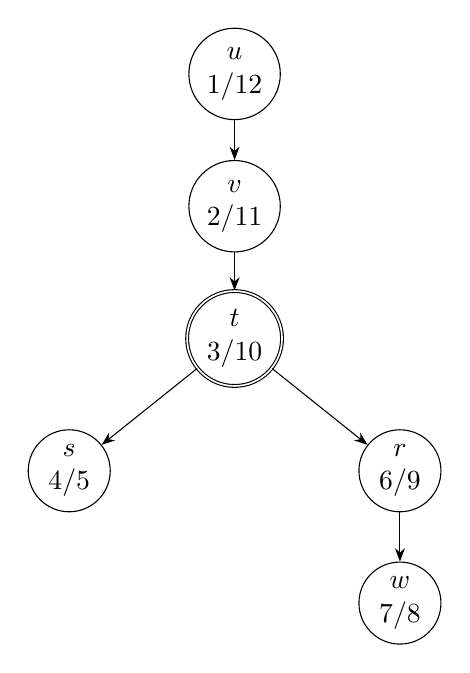
\begin{tikzpicture}[x=1.5cm,y=1.4cm]
\node[v](u)at(0,0){$u$\\$1/12$};\node[v](v)at(0,-1.2){$v$\\$2/11$};
\node[bf](t)at(0,-2.4){$t$\\$3/10$};\node[v](s)at(-1.4,-3.6){$s$\\$4/5$};
\node[v](r)at(1.4,-3.6){$r$\\$6/9$};\node[v](w)at(1.4,-4.8){$w$\\$7/8$};
\foreach\a/\b in{u/v,v/t,t/s,t/r,r/w}\draw[arr](\a)--(\b);
\end{tikzpicture}\end{center}
Labels: discovery/finish times; double circle: backtrack node.

Returns:
\[
s\rightsquigarrow t,\quad w\rightsquigarrow r\rightsquigarrow t\rightsquigarrow v\rightsquigarrow u.
\]
Backtrack node $=$ return point starting a new unvisited branch. $\boxed{bt=t}$.

$E_{\rm back}=\{(s,u),(w,v)\}$; all remaining edges are tree edges.

\newpage
\question{DFS2 (p.\ 3)}{Discovery and finish times}
Start $S$; alphabetical adjacency; right-hand graph. $D$ is one vertex, visited once.

Discovery order:
\[
\boxed{S,A,B,C,E,D,F,G}.
\]
Labels: discovery/finish times; double circles: backtrack nodes.
\begin{center}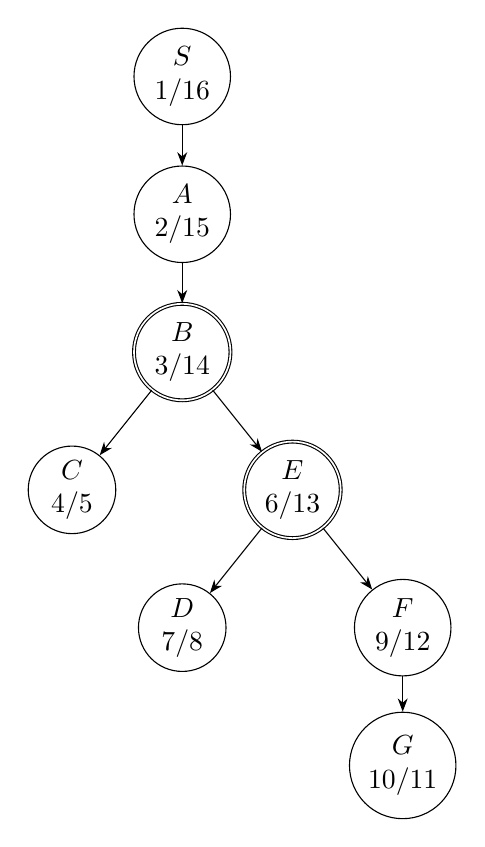
\begin{tikzpicture}[x=1.4cm,y=1.4cm]
\node[v](S)at(0,0){$S$\\$1/16$};\node[v](A)at(0,-1.25){$A$\\$2/15$};
\node[bf](B)at(0,-2.5){$B$\\$3/14$};
\node[v](C)at(-1,-3.75){$C$\\$4/5$};\node[bf](E)at(1,-3.75){$E$\\$6/13$};
\node[v](D)at(0,-5){$D$\\$7/8$};\node[v](F)at(2,-5){$F$\\$9/12$};\node[v](G)at(2,-6.25){$G$\\$10/11$};
\foreach\a/\b in{S/A,A/B,B/C,B/E,E/D,E/F,F/G}\draw[arr](\a)--(\b);
\end{tikzpicture}\end{center}
$\boxed{bt=\{B,E\}}$:
\[
C\rightsquigarrow B\to E,\qquad D\rightsquigarrow E\to F.
\]
$D\in\mathrm{visited}$ when $A,S$ resume: no second $D$ child.

\newpage
\question{DFS3 (p.\ 4)}{Continue after the dead end}
Keep the supplied prefix. Convention for remaining neighbors: ascending $rc$ labels ($rc=10r+c$). The grid slide gives no fixed directional order.

\textbf{1. Backtrack to $bf_1=41$:}
\[
(3,2)\rightsquigarrow(2,2)\rightsquigarrow(1,2)\rightsquigarrow(1,1)
\rightsquigarrow(2,1)\rightsquigarrow(3,1)\rightsquigarrow(4,1).
\]
Visit:
\[
(4,1)\to(5,1)\to(6,1)\to(6,2).
\]
$62$: dead end (all neighbors visited).

\textbf{2. Backtrack to $bf_2=42$:}
\[
(6,2)\rightsquigarrow(6,1)\rightsquigarrow(5,1)\rightsquigarrow(4,1)\rightsquigarrow(4,2).
\]
Visit:
\[
(4,2)\to(4,3)\to(4,4)\to(3,4)\to(2,4).
\]
$34<54$, so visit $34$ first; $24$ is a dead end.

\textbf{3. Backtrack to $bf_3=44$:}
\[
(2,4)\rightsquigarrow(3,4)\rightsquigarrow\boxed{bf_3=(4,4)}.
\]
$44\to54$: goal; stop. $\boxed{bf_1=41,\ bf_2=42,\ bf_3=44}$.

\begin{center}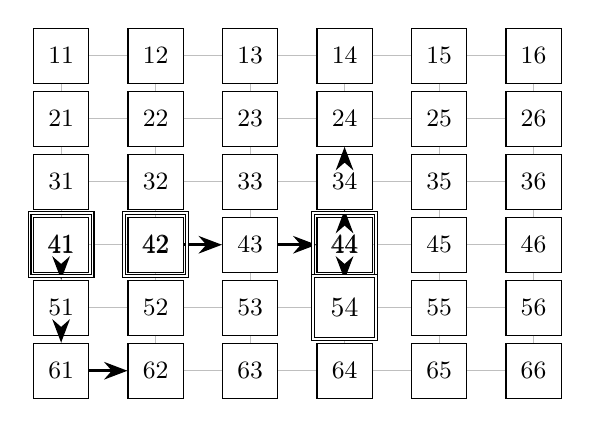
\begin{tikzpicture}[x=1.2cm,y=0.8cm]
\foreach\r in{1,...,6}\foreach\c in{1,...,6}{\node[draw,rectangle,minimum size=7mm,fill=white](n\r\c)at(\c,-\r){\small\r\c};}
\foreach\r in{1,...,6}\foreach\c in{1,...,5}{\pgfmathtruncatemacro{\d}{\c+1}\draw[gray!50](n\r\c)--(n\r\d);}
\foreach\r in{1,...,5}\foreach\c in{1,...,6}{\pgfmathtruncatemacro{\d}{\r+1}\draw[gray!50](n\r\c)--(n\d\c);}
\foreach\a/\b in{41/51,51/61,61/62,42/43,43/44,44/34,34/24,44/54}\draw[arr,very thick](n\a)--(n\b);
\node[draw,rectangle,minimum size=8mm,double]at(n41){41};\node[draw,rectangle,minimum size=8mm,double]at(n42){42};\node[draw,rectangle,minimum size=8mm,double]at(n44){44};
\node[draw,rectangle,minimum size=8mm,double,fill=white]at(n54){54};
\end{tikzpicture}\end{center}
Arrows: new visits. Double boxes: backtrack nodes and goal. Final path:
\begin{align*}
33\to23\to13\to14\to15\to25\to35\to45\to55\\
\to65\to64\to63\to53\to52\to42\to43\to44\to54.
\end{align*}


\newpage
\question{DFS4 (p.\ 5)}{DFS starting from $v$}
Start $v$; remaining roots and adjacency lists alphabetical.
\begin{center}\begin{tabular}{c|l@{\qquad}c|l}\toprule
Vertex&Outgoing neighbors&Vertex&Outgoing neighbors\\\midrule
$q$&$s,t,w$&$r$&$u,y$\\$s$&$v$&$t$&$x,y$\\$u$&$y$&$v$&$w$\\$w$&$s$&$x$&$z$\\$y$&$q$&$z$&$x$\\\bottomrule\end{tabular}\end{center}
Discovery order:
\[
\boxed{v,w,s,q,t,x,z,y,r,u}.
\]
DFS forest (discovery/finish times):
\begin{center}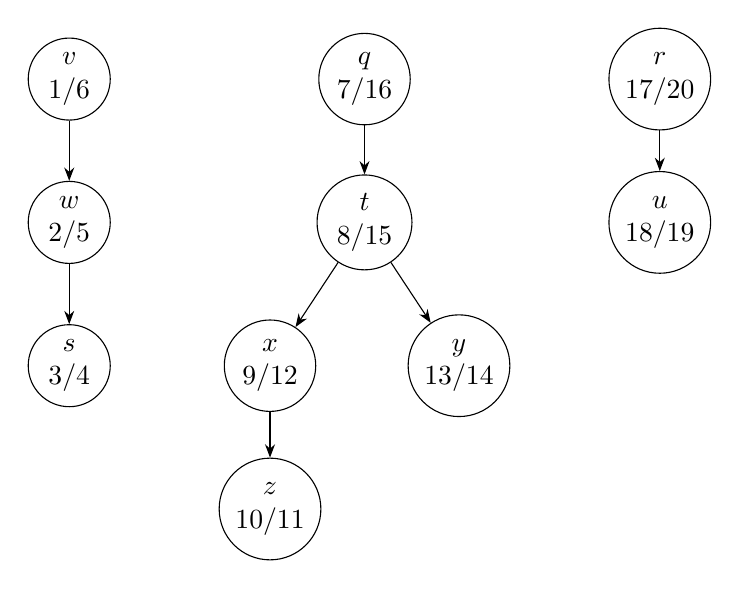
\begin{tikzpicture}[x=1.5cm,y=1.4cm]
\node[v](v)at(0,0){$v$\\$1/6$};\node[v](w)at(0,-1.3){$w$\\$2/5$};\node[v](s)at(0,-2.6){$s$\\$3/4$};
\node[v](q)at(2.5,0){$q$\\$7/16$};\node[v](t)at(2.5,-1.3){$t$\\$8/15$};
\node[v](x)at(1.7,-2.6){$x$\\$9/12$};\node[v](y)at(3.3,-2.6){$y$\\$13/14$};\node[v](z)at(1.7,-3.9){$z$\\$10/11$};
\node[v](r)at(5,0){$r$\\$17/20$};\node[v](u)at(5,-1.3){$u$\\$18/19$};
\foreach\a/\b in{v/w,w/s,q/t,t/x,x/z,t/y,r/u}\draw[arr](\a)--(\b);
\end{tikzpicture}\end{center}
Finish order: $s,w,v,z,x,y,t,q,u,r$. The non-tree edges are:
\begin{itemize}[nosep]
\item Back edges: $s\to v$, $z\to x$, $y\to q$.
\item Cross edges: $q\to s$, $q\to w$, $u\to y$, $r\to y$.
\end{itemize}
Roots: $v,q,r$.

\newpage
\question{DFS5 (p.\ 6)}{Topological ordering}
Reverse DFS finish order:
\[
\boxed{p,n,o,s,m,r,y,v,x,w,z,u,q,t}.
\]
Check: $(u,v)\in E\Rightarrow\operatorname{pos}(u)<\operatorname{pos}(v)$.
\begin{center}\begin{tabular}{c|l}\toprule
Vertex&Its outgoing neighbors, all later in the ordering\\\midrule
$p$&$o,s,z$\\$n$&$o,q,u$\\$o$&$r,s,v$\\$s$&$r$\\$m$&$q,r,x$\\$r$&$u,y$\\$y$&$v$\\$v$&$w,x$\\$w$&$z$\\$u$&$t$\\$q$&$t$\\\bottomrule\end{tabular}\end{center}
$t,x,z$: no outgoing edges.

\newpage
\question{Dijkstra1 (p.\ 7)}{Complete the shortest-path calculation}
Source $a$; $w(b,h)=1$. Initially $d(a)=0$, all other $d=\infty$.

$d(v)\leftarrow\min\{d(v),d(u)+w(u,v)\}$; settle minimum $d$ (alphabetical ties).
\begin{center}\small\begin{tabular}{c|c|rrrrrrrrr}\toprule
Step&Settled&$a$&$b$&$h$&$g$&$f$&$c$&$i$&$e$&$d$\\\midrule
0&--&0&$\infty$&$\infty$&$\infty$&$\infty$&$\infty$&$\infty$&$\infty$&$\infty$\\
1&$a$&0&4&8&$\infty$&$\infty$&$\infty$&$\infty$&$\infty$&$\infty$\\
2&$b$&0&4&5&$\infty$&$\infty$&12&$\infty$&$\infty$&$\infty$\\
3&$h$&0&4&5&6&$\infty$&12&12&$\infty$&$\infty$\\
4&$g$&0&4&5&6&8&12&12&$\infty$&$\infty$\\
5&$f$&0&4&5&6&8&12&12&18&22\\
6&$c$&0&4&5&6&8&12&12&18&19\\
7&$i$&0&4&5&6&8&12&12&18&19\\
8&$e$&0&4&5&6&8&12&12&18&19\\
9&$d$&0&4&5&6&8&12&12&18&19\\\bottomrule
\end{tabular}\normalsize\end{center}
Key relaxations:
\begin{align*}
d(g)&=d(h)+1=6,& d(i)&=d(h)+7=12,\\
d(f)&=d(g)+2=8,& d(e)&=d(f)+10=18,\\
d(d)&=d(f)+14=22\quad\text{initially},&&\\
d(d)&=\min(22,d(c)+7)=\min(22,19)=19.&&
\end{align*}
Final shortest-path tree:
\begin{center}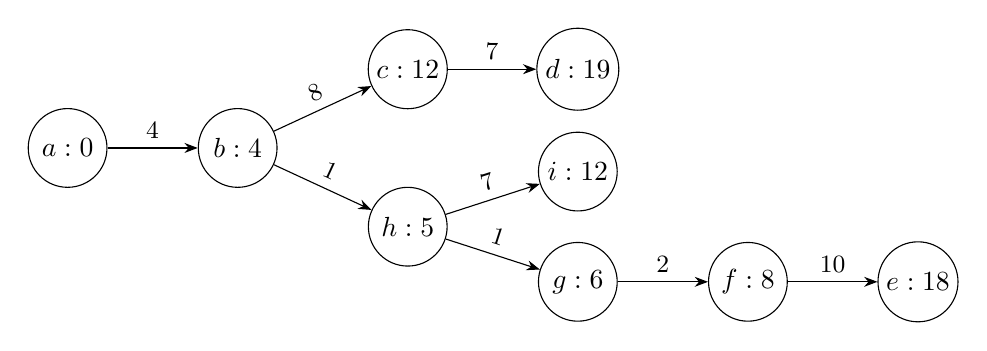
\begin{tikzpicture}[x=1.2cm,y=1cm]
\node[v](a)at(0,0){$a:0$};\node[v](b)at(1.8,0){$b:4$};\node[v](c)at(3.6,1){$c:12$};\node[v](d)at(5.4,1){$d:19$};
\node[v](h)at(3.6,-1){$h:5$};\node[v](i)at(5.4,-0.3){$i:12$};\node[v](g)at(5.4,-1.7){$g:6$};\node[v](f)at(7.2,-1.7){$f:8$};\node[v](e)at(9,-1.7){$e:18$};
\foreach\a/\b/\w in{a/b/4,b/c/8,c/d/7,b/h/1,h/i/7,h/g/1,g/f/2,f/e/10}\draw[arr](\a)--node[above,sloped]{\small\w}(\b);
\end{tikzpicture}\end{center}
Node labels: vertex and distance.

\newpage
\question{AStar1 (p.\ 8)}{A* with $h(B)=16$}
$f(n)=g(n)+h(n)$; $g=$ best known cost from $A$.
\[
\begin{array}{c|rrrrrrrrrr}
n&A&X&B&C&L&W&K&T&S&H\\\hline
h(n)&30&27&16&17&33&9&19&0&17&22
\end{array}
\]
$\mathrm{OPEN}=\{A(0,30)\}$. Notation $n(g,f)$; OPEN sorted by $f$.
\begin{center}\small\begin{tabular}{c|c|>{\raggedright\arraybackslash}p{6.4cm}|>{\raggedright\arraybackslash}p{4.4cm}}\toprule
Step&Pop&Calculations&OPEN after step\\\midrule
1&$A$&$g(X)=0+17=17$, $f(X)=17+27=44$&$X(17,44)$\\
2&$X$&$g(B)=17+16=33$, $f(B)=49$; $g(C)=17+11=28$, $f(C)=45$&$C(28,45)$, $B(33,49)$\\
3&$C$&$g(W)=28+11=39$, $f(W)=48$; $g(L)=28+20=48$, $f(L)=81$&$W(39,48)$, $B(33,49)$, $L(48,81)$\\
4&$W$&$g(T)=39+9=48$, $f(T)=48$; $g(K)=39+10=49$, $f(K)=68$;  $g(B):51>33$ (reject).&$T(48,48)$, $B(33,49)$, $K(49,68)$, $L(48,81)$\\
5&$T$&Goal popped; stop.&$B(33,49)$, $K(49,68)$, $L(48,81)$\\\bottomrule\end{tabular}\normalsize\end{center}
$\mathrm{CLOSED}: A,X,C,W,T$.
\[
\boxed{A\to X\to C\to W\to T},\qquad
\boxed{17+11+11+9=48}.
\]
\begin{center}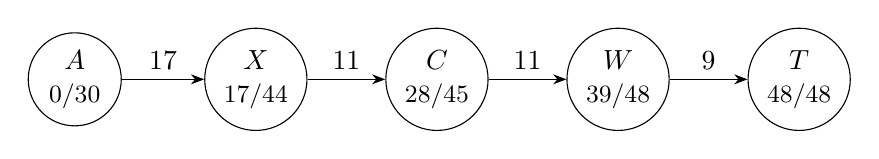
\begin{tikzpicture}[x=2.3cm]
\foreach\n/\x/\g/\f in{A/0/0/30,X/1/17/44,C/2/28/45,W/3/39/48,T/4/48/48}{\node[v](\n)at(\x,0){$\n$\\\small$\g/\f$};}
\foreach\a/\b/\w in{A/X/17,X/C/11,C/W/11,W/T/9}\draw[arr](\a)--node[above]{\w}(\b);
\end{tikzpicture}\end{center}
Node labels: $g/f$. Stop when the goal is popped.

\newpage
\question{AStar2 (p.\ 9)}{Change $h(B)$ from 16 to 6}
$h(B)=6$; relax and update OPEN entries and parents.
\begin{center}\small\begin{tabular}{c|c|>{\raggedright\arraybackslash}p{6.2cm}|>{\raggedright\arraybackslash}p{4.6cm}}\toprule
Step&Pop&Calculations&OPEN after step\\\midrule
1&$A$&$g(X)=17$, $f(X)=44$&$X(17,44)$\\
2&$X$&$g(B)=33$, $f(B)=33+6=39$; $g(C)=28$, $f(C)=45$&$B(33,39)$, $C(28,45)$\\
3&$B$&$g(W)=33+12=45$, $f(W)=54$; $g(T)=33+17=50$, $f(T)=50$; $g(S)=33+7=40$, $f(S)=57$&$C(28,45)$, $T(50,50)$, $W(45,54)$, $S(40,57)$\\
4&$C$&$g(W):45\to39$, $f(W)=48$, $p(W)=C$; $g(L)=48$, $f(L)=81$.&$W(39,48)$, $T(50,50)$, $S(40,57)$, $L(48,81)$\\
5&$W$&$g(T):50\to48$, $p(T)=W$; $g(K)=49$, $f(K)=68$; $g(B):51>33$ (reject).&$T(48,48)$, $S(40,57)$, $K(49,68)$, $L(48,81)$\\
6&$T$&Goal popped; stop.&$S(40,57)$, $K(49,68)$, $L(48,81)$\\\bottomrule\end{tabular}\normalsize\end{center}
Result:
\[
\boxed{A\to X\to C\to W\to T\text{ with cost }48}.
\]
Expansion order: $A,X,B,C,W,T$.

Without OPEN relaxation: $W(45,54)$ stays stale; $T(50,50)$ is popped, giving the wrong path $A\to X\to B\to T$ (cost $50>48$).

$h(B)\in\{6,16\}\le17=h^*(B)$: admissible. With $h(B)=6$, consistency fails:
\[
h(X)=27>16+h(B)=22,\qquad h(S)=17>7+h(B)=13.
\]
Inconsistent heuristic: reopen CLOSED if a better $g$ appears. This run needs only OPEN updates.

\newpage
\question{AStar3 (p.\ 10)}{Shortest paths among polygonal obstacles}
\textbf{(a)} Continuous positions: $\mathcal S\subset\mathbb R^2$, $\boxed{|\mathcal S|=\infty}$ (uncountable).

Visibility graph: vertices $S,G$ and obstacle corners; edges are unobstructed straight segments.
\[
5+3+4+4+4+3+6=29\text{ vertices}.
\]
$\boxed{|V_{\rm visibility}|=29+2=31}$ (reduced graph, not all physical positions).

\textbf{(b)} Triangle inequality: $|AC|\le|AB|+|BC|$ (strict for a non-collinear bend). Straighten free-space bends; essential bends occur at obstacle vertices.

Shortest path: straight segments through visible corners; some segments follow boundary edges.

\begin{center}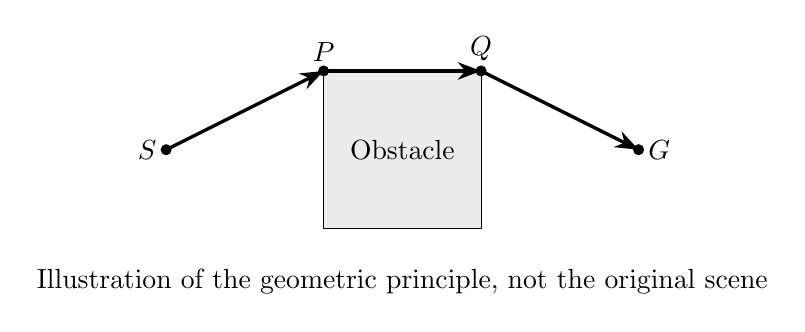
\begin{tikzpicture}[x=1cm,y=1cm]
\filldraw[fill=gray!15] (2,0)rectangle(4,2);
\coordinate(S)at(0,1);\coordinate(G)at(6,1);\coordinate(P)at(2,2);\coordinate(Q)at(4,2);
\draw[very thick,arr](S)--(P);\draw[very thick,arr](P)--(Q);\draw[very thick,arr](Q)--(G);
\fill(S)circle(2pt)node[left]{$S$};\fill(G)circle(2pt)node[right]{$G$};\fill(P)circle(2pt)node[above]{$P$};\fill(Q)circle(2pt)node[above]{$Q$};
\node at(3,1){Obstacle};\node[below]at(3,-0.4){Illustration of the geometric principle, not the original scene};
\end{tikzpicture}\end{center}
Assume a point robot, Euclidean distance, boundary contact allowed.
\end{document}
